% !TEX root = ../my-thesis.tex
%
\chapter{Supporting material for Chapter \ref{sec:comparison}}
\label{sec:appendix}


\section{ADQL query used to download data}\label{app:c2:adql}

 \emph{Gaia}  DR2 data for this work was downloaded with the following ADQL query. \texttt{\{start\_number\}} should be replaced with the first possible \texttt{source\_id} of the desired pixel using Eqn.~\ref{c2:eqn:healpix}. \texttt{\{end\_number\}} should be replaced with the first possible \texttt{source\_id} of the next integer pixel.

\begin{verbatim}
SELECT
-- Gaia astrometry
g.source_id, g.l, g.b, 
g.ra, g.ra_error, g.dec, g.dec_error, 
g.parallax, g.parallax_error, 
g.parallax_over_error, 
g.pmra, g.pmra_error, g.pmdec, g.pmdec_error, 
g.astrometric_params_solved, 

-- Gaia photometry
g.phot_g_mean_mag, g.phot_g_mean_flux, 
g.phot_g_mean_flux_error, 
g.phot_bp_mean_mag, g.phot_bp_mean_flux, 
g.phot_bp_mean_flux_error, 
g.phot_rp_mean_mag, g.phot_rp_mean_flux, 
g.phot_rp_mean_flux_error, 
g.phot_bp_rp_excess_factor, 

-- Calculate HEALPix level 5 index
GAIA_HEALPIX_INDEX(5, g.source_id) 
  AS gaia_healpix_5, 
               
-- RUWE statistics
r.ruwe, 
               
-- CBJ+2018 distances
d.r_est, d.r_lo, d.r_hi, 
d.r_len, d.result_flag 
               
-- Inner join the tables
FROM gaiadr2.gaia_source AS g 
INNER JOIN 
  gaiadr2.ruwe 
  AS r 
  ON g.source_id = r.source_id 
INNER JOIN 
  external.gaiadr2_geometric_distance 
  AS d 
  ON g.source_id = d.source_id 
           
-- Select only valid points
WHERE g.source_id >= {start_number} 
AND g.source_id < {end_number} 
AND g.astrometric_params_solved=31 
AND g.phot_bp_mean_mag IS NOT NULL 
AND g.phot_rp_mean_mag IS NOT NULL
\end{verbatim}


%-------------------------------------------------------------------
\section{Comparison with other OC catalogues}\label{app:c2:comparison_with_cats}

We present brief comparisons with the results of other OC catalogues, in lieu of best practices proposed in \cite{cantat-gaudin_clusters_2020} and as a part of efforts towards generally improving the quality of the OC census, reporting on both positive and negative detections. In future works, we hope to expand comparisons such as this across the entire OC census, offering another viewpoint on the existence of many literature OCs.


\subsection{\cite{cantat-gaudin_clusters_2020}}

Of the 537 objects listed in \cite{cantat-gaudin_clusters_2020} and in the fields in this study, we are able to detect 86.4\% of them with at least one algorithm or parameter combination, many of which are clear overdensities with well-resolved parameters.

We single out Auner 1, Berkeley 91 and Patchick 75 from Sect.~\ref{c2:sec:analysis_results} as objects that should be detectable but are not found by any algorithm. In addition, FSR 1460 and FSR 1509 are also undetected. If real, these objects are distant and difficult to detect in \emph{Gaia} data, although these objects also have heavily polluted CMDs in the membership lists of \cite{cantat-gaudin_clusters_2020} and hence may simply be associations. Future \emph{Gaia} data releases with better astrometric precision will shed more light on the status of these edge-case objects.


\subsection{MWSC}

We concur with the results of \cite{cantat-gaudin_gaia_2018} and \cite{cantat-gaudin_clusters_2020} that a majority of the objects in MWSC are undetectable in \emph{Gaia} data. Some of these objects may simply not be visible in \emph{Gaia} data due to reddening or large distances, although many are also likely to not be real. Future studies will have to quantify this for all OCs on a case-by-case basis. Of our 100 main OCs that were randomly selected from the MWSC catalogue, we detected OCs corresponding to 35 of them, suggesting that $\approx$35\% of the total MWSC catalogue is visible in \emph{Gaia} data. 

However, our results show that a number of MWSC objects appear to have been missed by works such as \cite{cantat-gaudin_clusters_2020}. In our larger crossmatching effort, we recovered candidates corresponding to 193 of the 607 objects listed in MWSC (31.8\%) but that are undetected in \cite{cantat-gaudin_clusters_2020}. Some of these objects may be new OCs that happen to have similar parameters to old objects, although some others are new detections of MWSC OCs in \emph{Gaia} data.

The best examples of re-detected OCs were Collinder 347, FSR 0124, FSR 0270 and FSR 1406, which were were clearly crossmatched and are clearly visible by eye in \emph{Gaia} data. In addition, Collinder 347 has also been well detected by \cite{piatti_extended_2019} in \emph{Gaia} DR2 data and recently by \cite{claria_ccd_2019} in visual spectrum photometric data. The sparse OCs Sgr OB6, Sgr OB7 and ASCC 100 were also detected, the latter of which has few members but is nearby with a parallax of 2.75 mas, suggesting that some OCs are yet to be recovered in \emph{Gaia} data even at small distances. In all seven cases, the crossmatched objects were clearly compatible in positional and distance space with MWSC values. They are also compatible in proper motion space, although at large distances the PPMXL proper motions in MWSC provide very little constraint.

While the catalogue of \cite{cantat-gaudin_clusters_2020} is the most complete and homogeneous OC catalogue to date, it still appears to lack some OCs from the literature and contains a handful of OCs that are somewhat putative. Ongoing comparisons with the results of multiple different clustering algorithms and methodologies will help to confirm, question or deny the existence of more OCs in the literature.


\subsection{\cite{castro-ginard_hunting_2020} and \cite{liu_catalog_2019}}

\cite{castro-ginard_hunting_2020} and \cite{liu_catalog_2019} have recently reported a combined total of over 600 new OCs in \emph{Gaia} DR2 data respectively. Of the \review{209 }objects from \cite{castro-ginard_hunting_2020} in the fields in this study, we detected OCs compatible with \review{135 }of them (\review{64.6}\%), representing a \review{sizable }fraction of their catalogue of new OCs that has been detected independently in \emph{Gaia} data for the first time. We note that the undetected OC UBC 638 is very close to UBC 637 (which is detected) - their reported centres are within 0.05$^{\circ}$ of one another, their proper motions 0.07 mas yr$^{-1}$ and parallaxes to within 0.1 mas, so they may be the same object.

We are able to detect OCs compatible with 24 of the 32 OCs from the catalogue of \cite{liu_catalog_2019} that are included in this study. The reasons for non-detections of OCs from both of these works remain unclear, and would need to be investigated in a future study.



%-------------------------------------------------------------------
\section{\review{Tables of detected clusters and members}}\label{app:c2:extra_tables}

\review{Four supplementary tables are available in online-only material at the CDS}\footnote{\href{https://vizier.u-strasbg.fr/}{https://vizier.u-strasbg.fr/}}\review{. For literature clusters, all detections by all algorithms are listed following the same format as Table~\ref{app:c2:tab:cluster_lists}.1. Any one cluster may have up to 12 different entries from detections by different algorithm and parameter combinations. When no detections were made of a literature cluster, a single blank row is given with only columns one and 26 filled. The 41 new objects have their mean parameters listed in a separate table following the format of Table~\ref{app:c2:tab:cluster_lists}.1 except with column 26 omitted.} \review{For both literature and new OCs, members are listed in tables following the format of Table~\ref{app:c2:tab:cluster_members}.2.}

% Cluster lists table
\begin{table}
\caption{\review{Description of the tables of detected OCs.}}
\label{app:c2:tab:cluster_lists}
\centering
\begin{tabular}{c c c l}
\hline\hline
\review{Col. }& \review{Label }& \review{Unit }& \review{Description }\\
\hline                        
\review{1     }& \review{Name                  }& \review{--  }& \review{Designation }\\
\review{2     }& \review{Internal ID           }& \review{--  }& \review{Internal designation }\\
\review{3     }& \review{Algorithm             }& \review{--  }& \review{Algorithm for detection }\\
\review{4     }& \review{Parameters            }& \review{--  }& \review{Algorithm parameters }\\
\review{5-7}\tablefootmark{a}   & \review{$\alpha$ }& \review{deg }& \review{Right ascension }\\
\review{8-10}\tablefootmark{a}  & \review{$\delta$ }& \review{deg }& \review{Declination }\\
\review{11    }& \review{$l$                   }& \review{deg }& \review{Galactic longitude }\\
\review{12    }& \review{$b$                   }& \review{deg }& \review{Galactic latitude }\\
\review{13-15}\tablefootmark{a} & \review{$\mu_{\alpha^*}$ }& \review{mas yr$^{-1}$ }& \review{Prop. motion in $\alpha \cdot \cos \delta$ }\\
\review{16-18}\tablefootmark{a} & \review{$\mu_\delta$ }& \review{mas yr$^{-1}$ }& \review{Prop. motion in $\delta$ }\\
\review{19-21}\tablefootmark{a} & \review{$\varpi$ }& \review{mas }& \review{Parallax }\\
\review{22    }& \review{$r_{50}$              }& \review{deg }& \review{Radius containing  }\\
      &                       &     & \review{50\% of members }\\
\review{23    }& \review{$r_t$                 }& \review{deg }& \review{Estimated tidal radius}\tablefootmark{b} \\
\review{24    }& \review{$n$                   }& \review{--  }& \review{Number of members }\\
\review{25    }& \review{$\sigma_{\text{CST}}$ }& \review{--  }& \review{CST score }\\
\review{26    }& \review{Source                }& \review{--  }& \review{Source catalogue }\\
\hline

\end{tabular}

\tablefoot{
\tablefoottext{a}{Where marked, three columns are provided: the mean value, standard deviation $\sigma$, and standard error $\sigma \, / \sqrt{n}$.}
\tablefoottext{b}{Estimated using the maximum distance between the centre of the cluster and an identified member star.}
}

\end{table}

% Cluster members table
\begin{table}
\caption{\review{Description of the membership tables for detected OCs.}}
\label{app:c2:tab:cluster_members}
\centering
\begin{tabular}{c c c l}
\hline\hline
\review{Col. }& \review{Label }& \review{Unit }& \review{Description }\\
\hline
\review{1     }& \review{Name                  }& \review{--  }& \review{Designation }\\
\review{2     }& \review{Internal ID           }& \review{--  }& \review{Internal designation }\\
\review{3     }& \review{Algorithm             }& \review{--  }& \review{Algorithm for detection }\\
\review{4     }& \review{Parameters            }& \review{--  }& \review{Algorithm parameters }\\
\review{5     }& \review{Source ID             }& \review{--  }& \emph{\review{Gaia}} \review{DR2 source ID }\\
\review{6-7}\tablefootmark{a} & \review{$\alpha$ }& \review{deg }& \review{Right ascension }\\
\review{8-9}\tablefootmark{a} & \review{$\delta$ }& \review{deg }& \review{Declination }\\
\review{10    }& \review{$l$                   }& \review{deg }& \review{Galactic longitude }\\
\review{11    }& \review{$b$                   }& \review{deg }& \review{Galactic latitude }\\
\review{12-13}\tablefootmark{a} & \review{$\mu_{\alpha^*}$ }& \review{mas yr$^{-1}$ }& \review{Prop. motion in $\alpha \cdot \cos \delta$ }\\
\review{14-15}\tablefootmark{a} & \review{$\mu_\delta$ }& \review{mas yr$^{-1}$ }& \review{Prop. motion in $\delta$ }\\
\review{16-17}\tablefootmark{a} & \review{$\varpi$ }& \review{mas }& \review{Parallax }\\
\review{18    }& \review{Gmag                  }& \review{mag }& \review{G-band magnitude  }\\
\review{19    }& \review{BPmag                 }& \review{mag }& \review{BP-band magnitude }\\
\review{20    }& \review{RPmag                 }& \review{mag }& \review{RP-band magnitude }\\
\review{21-22}\tablefootmark{a}& \review{G flux}& \review{$e^{-1}$ s$^{-1 }$}& \review{G-band flux}\\
\review{23-24}\tablefootmark{a}& \review{BP flux}& \review{$e^{-1}$ s$^{-1 }$}& \review{BP-band flux}\\
\review{25-26}\tablefootmark{a}& \review{RP flux}& \review{$e^{-1}$ s$^{-1 }$}& \review{RP-band flux}\\
\review{27}\tablefootmark{b}& \review{$p$}& \review{--  }& \review{Membership probability}\\
\hline

\end{tabular}

\tablefoot{
\tablefoottext{a}{Where marked, two columns are provided: the mean value and the standard error.}
\tablefoottext{b}{Always equal to one for DBSCAN as it does not produce membership probabilities for individual stars.}
}

\end{table}

%-------------------------------------------------------------------
\section{\reviewtwo{Plots of newly detected OCs}}\label{app:c2:new_oc_plots}

See Figs.~\ref{app:c2:fig:new_ocs_0}, \ref{app:c2:fig:new_ocs_1}, \ref{app:c2:fig:new_ocs_2}, \ref{app:c2:fig:new_ocs_3}, \ref{app:c2:fig:new_ocs_4}, \ref{app:c2:fig:new_ocs_5}, and \ref{app:c2:fig:new_ocs_6}.

\begin{figure*}[ht]
   \centering
   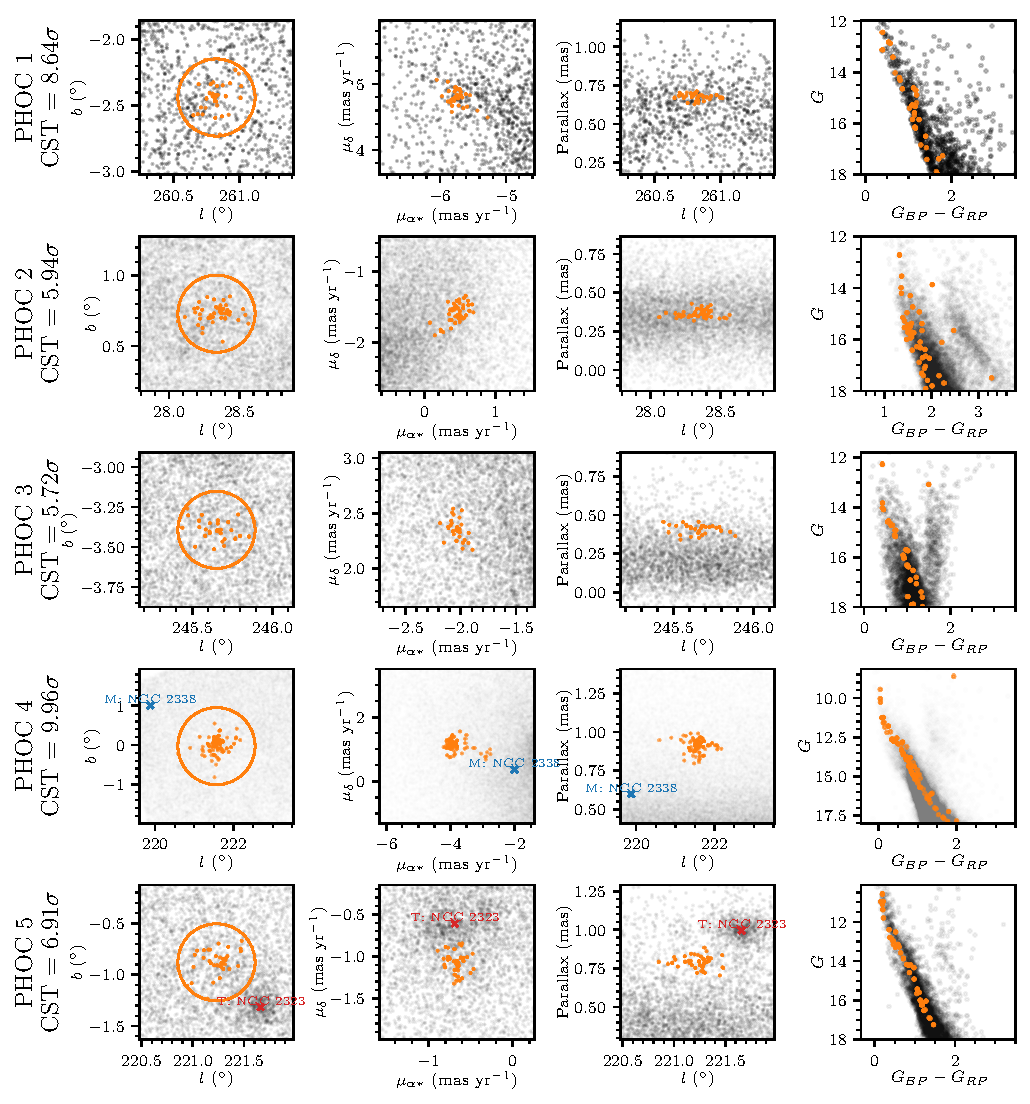
\includegraphics[width=\textwidth]{fig/c2/fig_new_ocs_0.pdf}
   \caption[Plots of the new OCs PHOC 1 to 5]{\reviewtwo{Astrometric and photometric plots of the first five new OCs from Sect.~\ref{c2:sec:new_ocs}. Identified member stars are shown in orange, with background stars in black. Only members with a membership probability of greater than 50\% are plotted. The estimated tidal radius for the OCs is depicted with a circle in the $l$ vs. $b$ plots in the first column. CST scores for each object are shown with its name on the left. Nearby OCs from literature catalogues are marked when visible. T (in red text) denotes sources from \cite{cantat-gaudin_clusters_2020}, while M (blue) and S (purple) denote sources from MWSC and \cite{sim_207_2019} respectively that were not detected by \cite{cantat-gaudin_clusters_2020}. A (brown) denotes new OCs detected recently by \cite{castro-ginard_hunting_2020}.   }}\label{app:c2:fig:new_ocs_0}%
\end{figure*}


\begin{figure*}[ht]
   \centering
   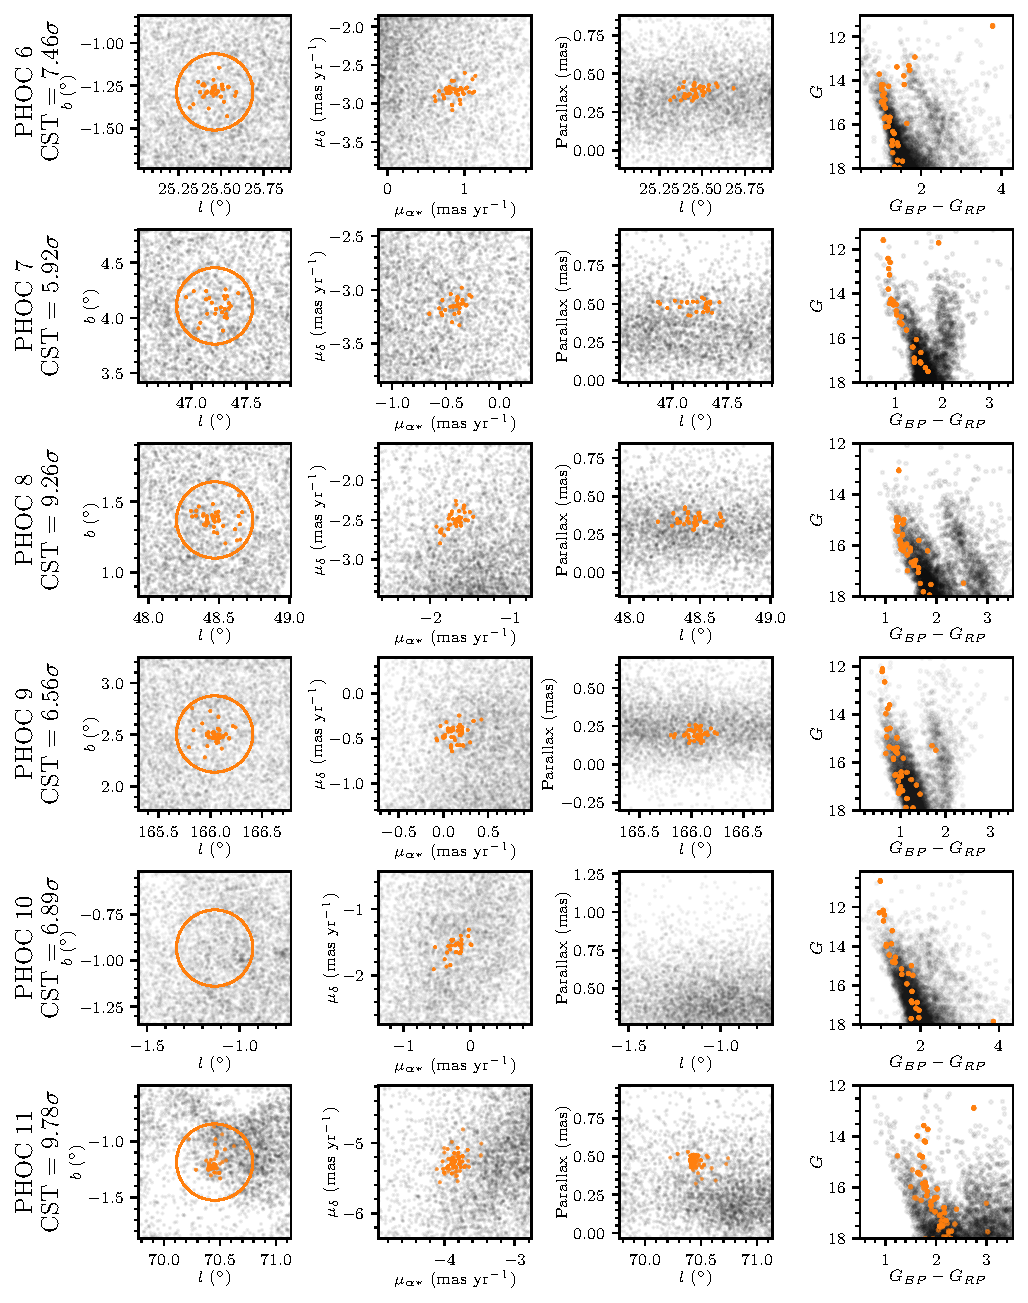
\includegraphics[width=\textwidth]{fig/c2/fig_new_ocs_1.pdf}
   \caption[Plots of the new OCs PHOC 6 to 11]{\reviewtwo{Plots of the new OCs PHOC 6 to 11, plotted in the same style as Fig.~\ref{app:c2:fig:new_ocs_0}. }}%
   \label{app:c2:fig:new_ocs_1}
\end{figure*}

\begin{figure*}[ht]
   \centering
   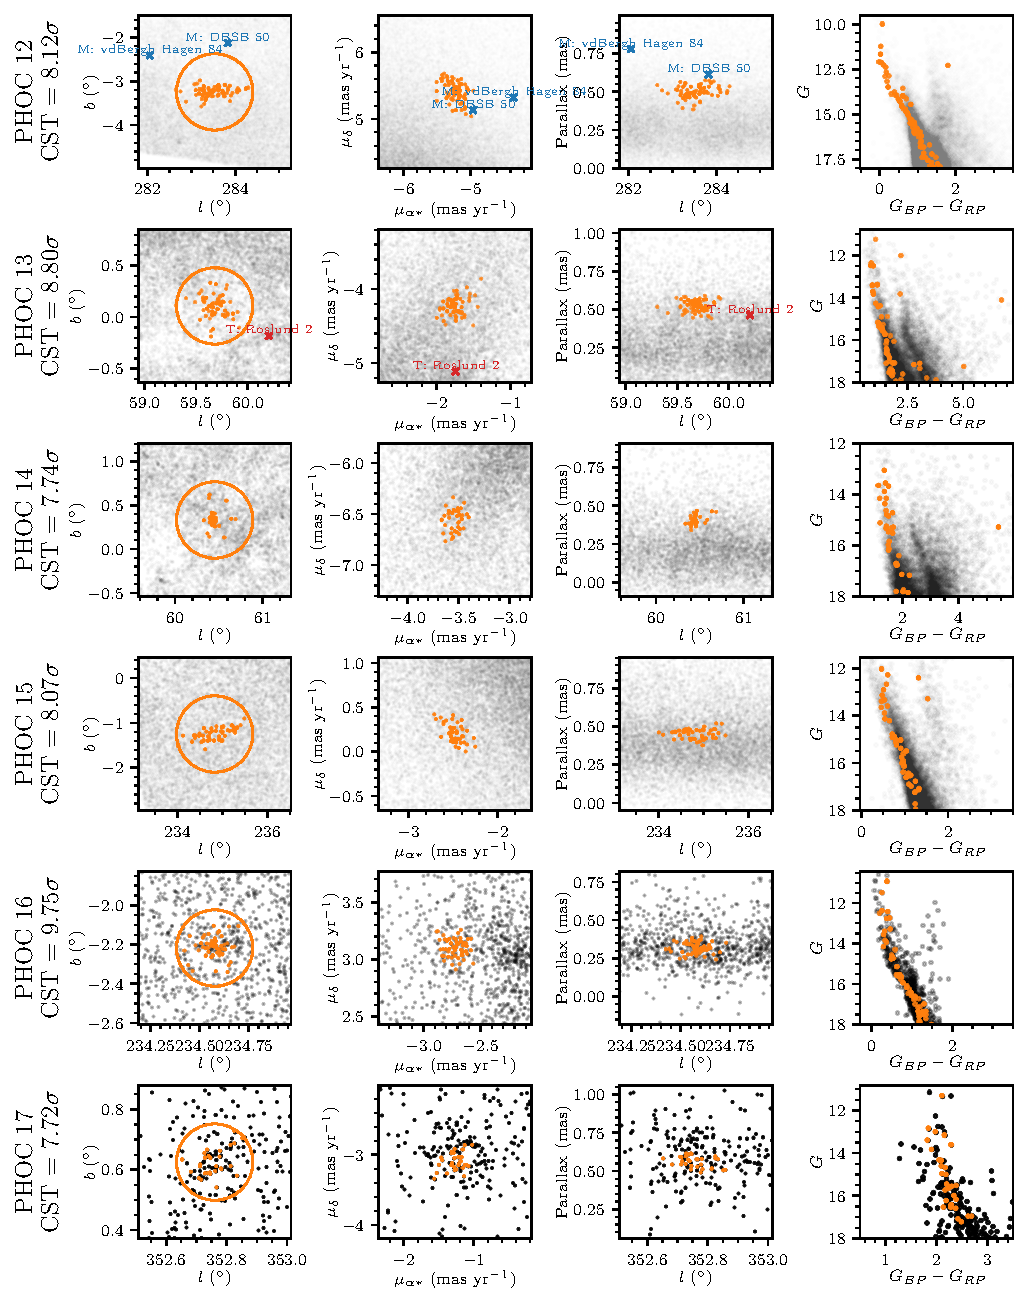
\includegraphics[width=\textwidth]{fig/c2/fig_new_ocs_2.pdf}
   \caption[Plots of the new OCs PHOC 12 to 17]{\reviewtwo{Plots of the new OCs PHOC 12 to 17, plotted in the same style as Fig.~\ref{app:c2:fig:new_ocs_0}. }}%
   \label{app:c2:fig:new_ocs_2}
\end{figure*}

\begin{figure*}[ht]
   \centering
   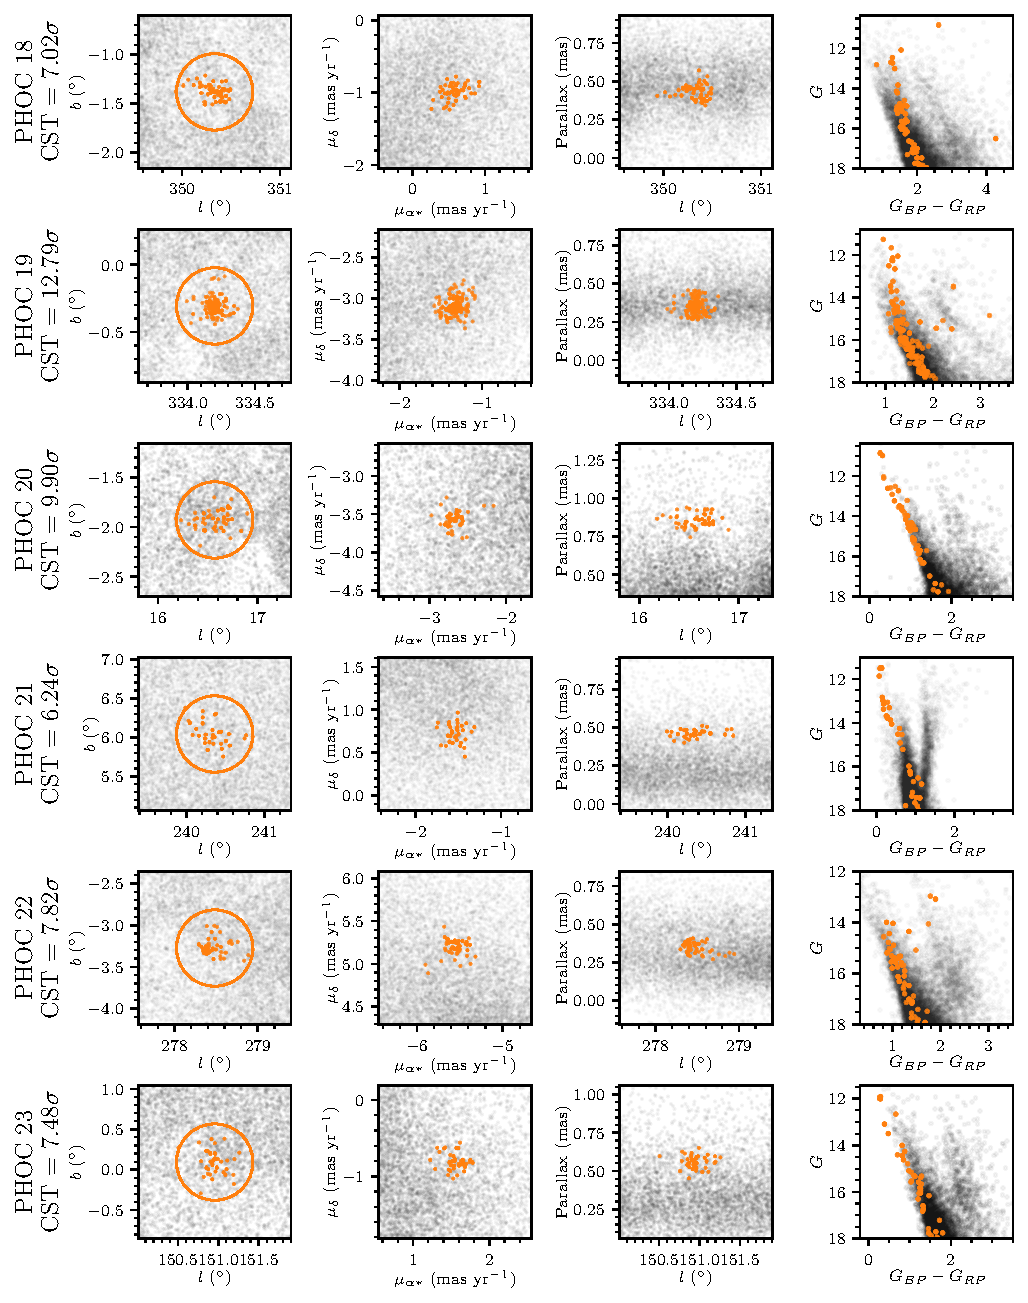
\includegraphics[width=\textwidth]{fig/c2/fig_new_ocs_3.pdf}
   \caption[Plots of the new OCs PHOC 18 to 23]{\reviewtwo{Plots of the new OCs PHOC 18 to 23, plotted in the same style as Fig.~\ref{app:c2:fig:new_ocs_0}. }}%
   \label{app:c2:fig:new_ocs_3}
\end{figure*}

\begin{figure*}[ht]
   \centering
   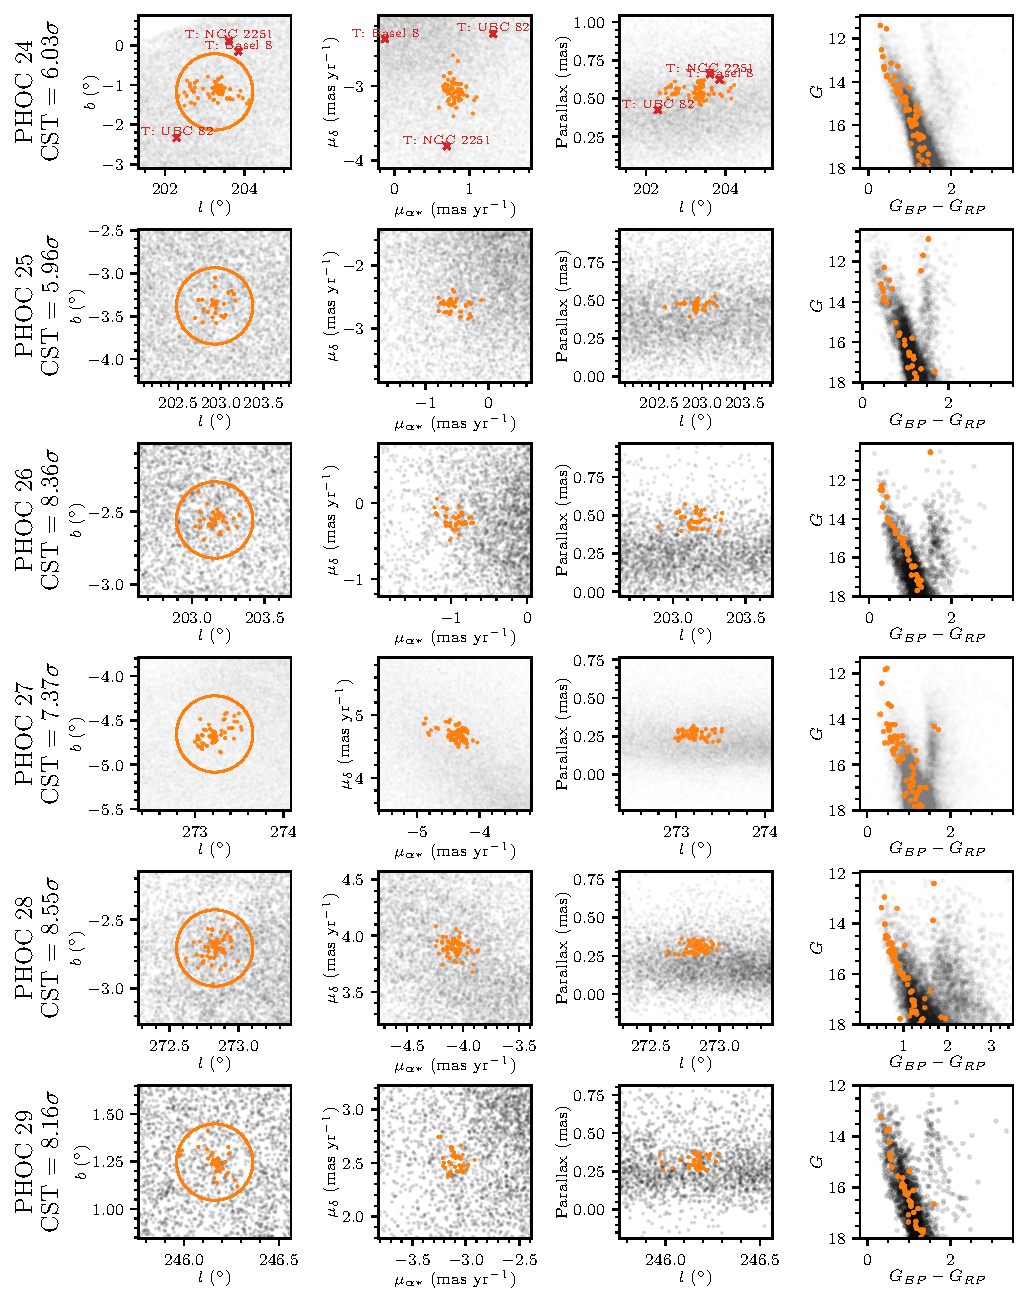
\includegraphics[width=\textwidth]{fig/c2/fig_new_ocs_4.pdf}
   \caption[Plots of the new OCs PHOC 24 to 29]{\reviewtwo{Plots of the new OCs PHOC 24 to 29, plotted in the same style as Fig.~\ref{app:c2:fig:new_ocs_0}. }}%
   \label{app:c2:fig:new_ocs_4}
\end{figure*}

\begin{figure*}[ht]
   \centering
   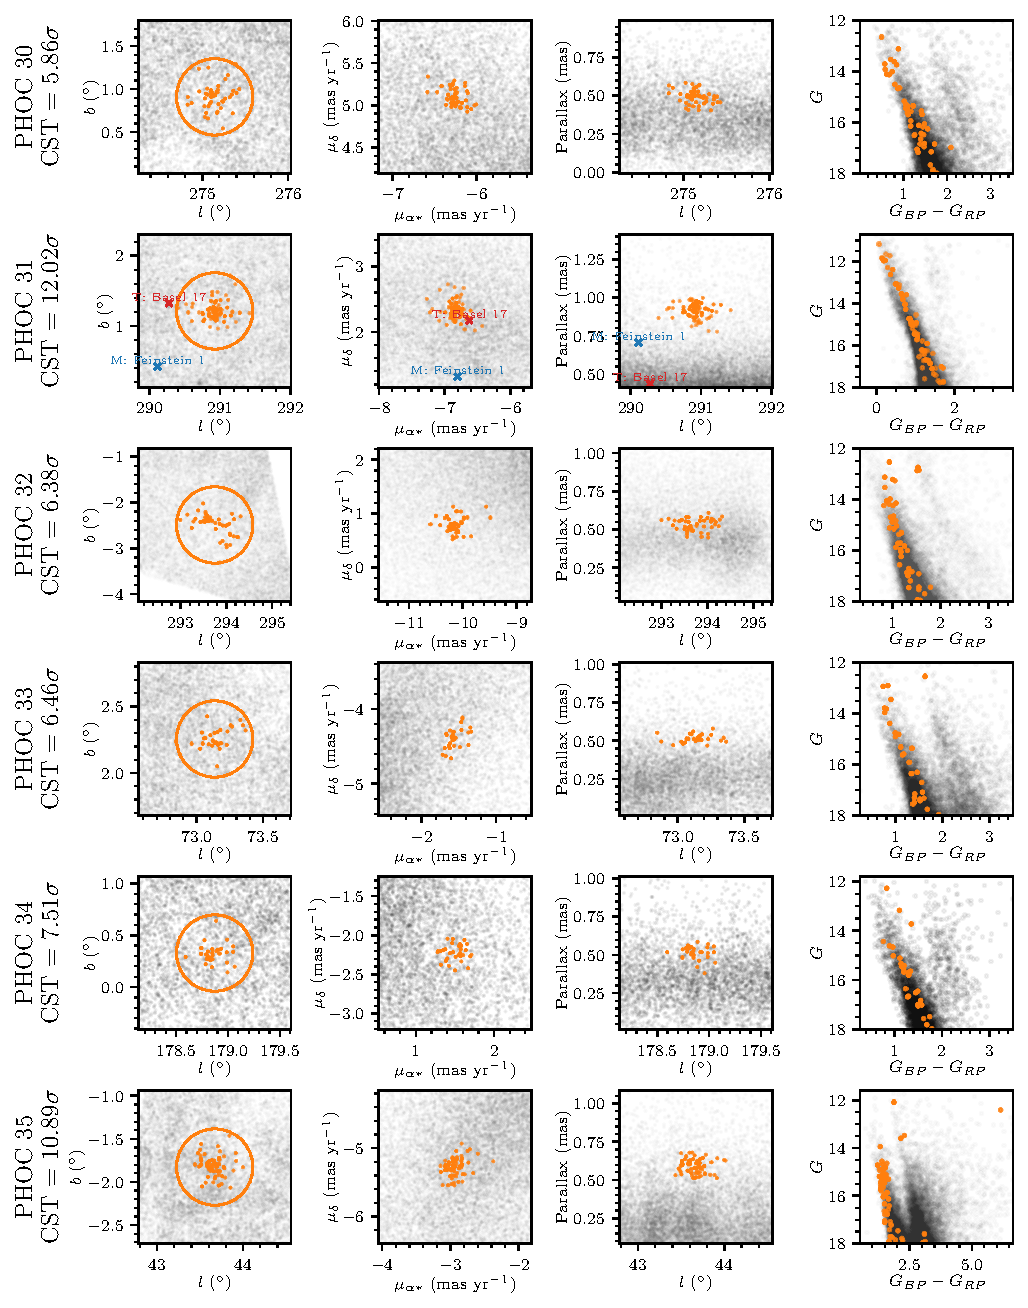
\includegraphics[width=\textwidth]{fig/c2/fig_new_ocs_5.pdf}
   \caption[Plots of the new OCs PHOC 30 to 35]{\reviewtwo{Plots of the new OCs PHOC 30 to 35, plotted in the same style as Fig.~\ref{app:c2:fig:new_ocs_0}. }}%
   \label{app:c2:fig:new_ocs_5}
\end{figure*}

\begin{figure*}[ht]
   \centering
   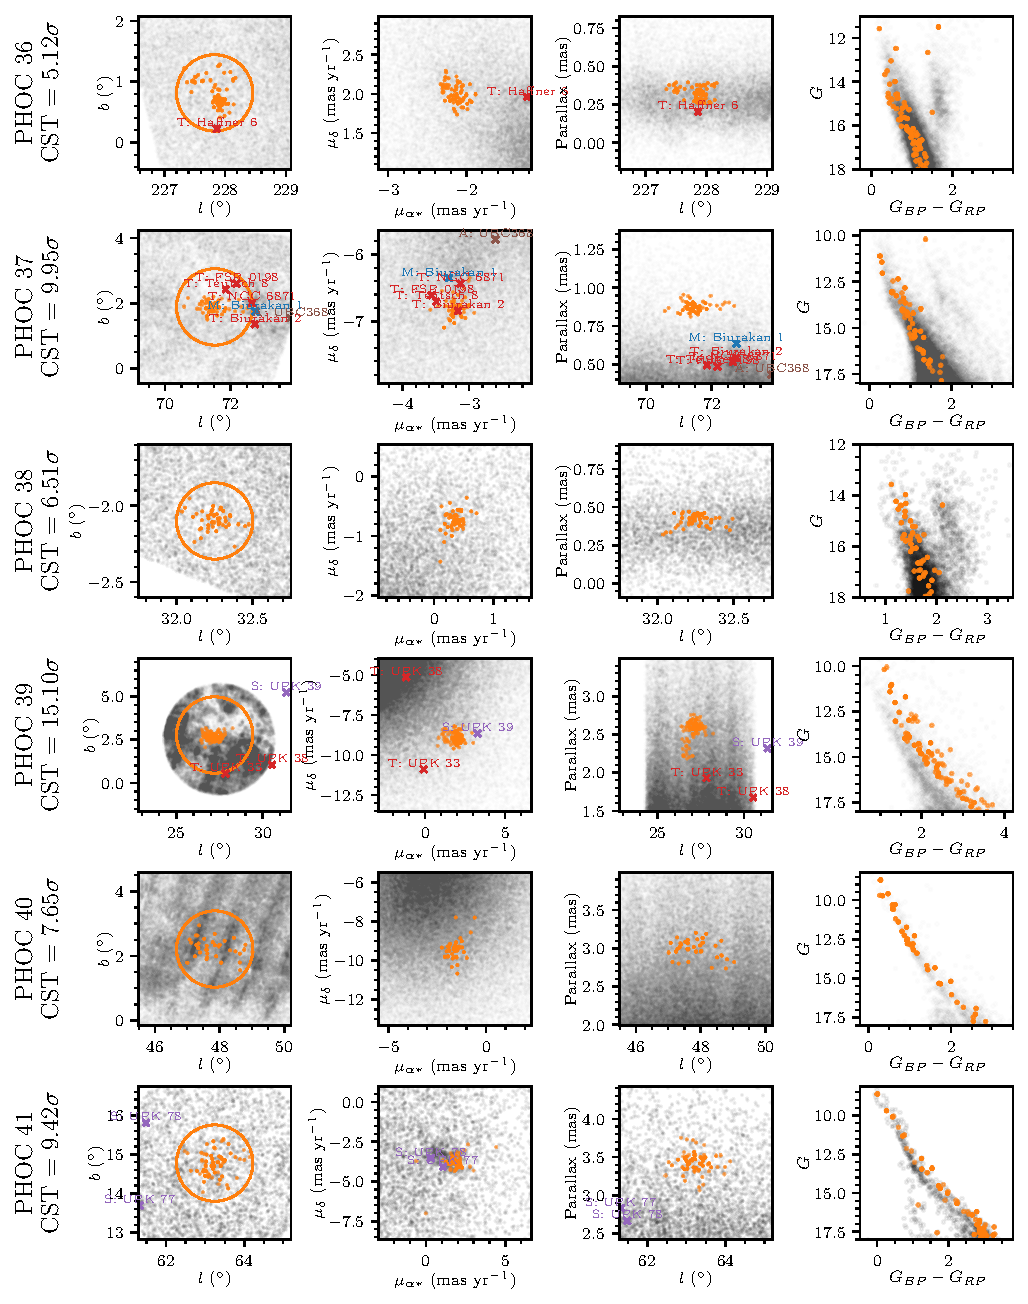
\includegraphics[width=\textwidth]{fig/c2/fig_new_ocs_6.pdf}
   \caption[Plots of the new OCs PHOC 36 to 41]{\reviewtwo{Plots of the new OCs PHOC 36 to 41, plotted in the same style as Fig.~\ref{app:c2:fig:new_ocs_0}. }}%
   \label{app:c2:fig:new_ocs_6}
\end{figure*}




%-------------------------------------------------------------------


\section{List of fields used in this study}\label{app:c2:fields}

See Table \ref{app:c2:table:sky_locations}.

\begin{table*}

% Define first header
\caption{\label{app:c2:table:sky_locations}Sky locations and HEALPix indices of the central pixels included in this study.}

\centering
\footnotesize
\begin{tabular}{cccc|cccc}
\hline\hline
Number & $\alpha$ ($^\circ$) & $\delta$ ($^\circ$) & Pixel\tablefootmark{a} & Number & $\alpha$ ($^\circ$) & $\delta$ ($^\circ$) & Pixel\tablefootmark{a} \\
\hline

0  & 313.6 & -12.0 & 12238 & 50 & 318.1 & 46.6  & 3844  \\
1  & 104.1 & 18.2  & 5976  & 51 & 91.4  & 30.0  & 6106  \\
2  & 128.0 & -41.8 & 9817  & 52 & 136.9 & -54.3 & 9434  \\
3  & 343.9 & 69.4  & 3953  & 53 & 357.6 & 61.9  & 3575  \\
4  & 90.0  & 6.0   & 5900  & 54 & 48.1  & 46.6  & 772   \\
5  & 281.2 & -3.6  & 7564  & 55 & 76.5  & 45.0  & 365   \\
6  & 99.8  & 9.6   & 5909  & 56 & 120.9 & -31.4 & 9940  \\
7  & 92.8  & -6.0  & 5364  & 57 & 278.4 & -23.3 & 7243  \\
8  & 98.4  & 6.0   & 5563  & 58 & 293.9 & 22.0  & 3585  \\
9  & 281.2 & -25.9 & 7235  & 59 & 143.7 & -51.3 & 9437  \\
10 & 113.9 & -30.0 & 9946  & 60 & 34.4  & 64.9  & 915   \\
11 & 61.9  & 40.2  & 403   & 61 & 246.1 & -27.3 & 10738 \\
12 & 225.0 & -64.9 & 10432 & 62 & 274.2 & -17.0 & 7278  \\
13 & 106.9 & -8.4  & 5420  & 63 & 169.3 & -58.9 & 9484  \\
14 & 281.2 & -8.4  & 7552  & 64 & 84.4  & 31.4  & 6124  \\
15 & 73.1  & 31.4  & 284   & 65 & 168.2 & -61.9 & 9480  \\
16 & 286.9 & 13.2  & 7663  & 66 & 325.8 & 52.8  & 3860  \\
17 & 80.2  & 41.8  & 346   & 67 & 246.1 & -32.8 & 10702 \\
18 & 78.8  & 48.1  & 378   & 68 & 321.1 & 57.4  & 3870  \\
19 & 268.6 & -30.0 & 7205  & 69 & 302.3 & 35.7  & 3657  \\
20 & 303.8 & 34.2  & 3651  & 70 & 116.7 & -17.0 & 10158 \\
21 & 152.1 & -58.9 & 9340  & 71 & 88.6  & 27.3  & 6094  \\
22 & 120.9 & -10.8 & 5396  & 72 & 272.8 & -31.4 & 7192  \\
23 & 316.6 & 48.1  & 3846  & 73 & 85.8  & 30.0  & 6118  \\
24 & 295.3 & 23.3  & 3588  & 74 & 203.6 & -58.9 & 10427 \\
25 & 319.2 & 35.7  & 3317  & 75 & 48.6  & 52.8  & 792   \\
26 & 357.0 & 67.9  & 3927  & 76 & 315.0 & 46.6  & 3843  \\
27 & 112.5 & -20.7 & 9983  & 77 & 274.2 & 30.0  & 8153  \\
28 & 143.4 & -31.4 & 10004 & 78 & 112.5 & -18.2 & 5376  \\
29 & 272.8 & -18.2 & 7275  & 79 & 299.5 & 30.0  & 3606  \\
30 & 299.5 & 35.7  & 3658  & 80 & 289.7 & 10.8  & 7655  \\
31 & 136.6 & -48.1 & 9462  & 81 & 307.8 & 52.8  & 3875  \\
32 & 157.5 & -57.4 & 9506  & 82 & 98.4  & 23.3  & 6008  \\
33 & 257.3 & -38.7 & 10610 & 83 & 111.1 & -14.5 & 5385  \\
34 & 36.6  & 66.4  & 918   & 84 & 285.5 & 32.8  & 3630  \\
35 & 261.6 & -37.2 & 10612 & 85 & 255.9 & -37.2 & 10616 \\
36 & 204.8 & -60.4 & 10425 & 86 & 272.8 & -8.4  & 7387  \\
37 & 245.0 & -49.7 & 10543 & 87 & 300.9 & 34.2  & 3656  \\
38 & 258.8 & -37.2 & 10611 & 88 & 272.8 & -20.7 & 7272  \\
39 & 310.8 & 12.0  & 3117  & 89 & 23.8  & 64.9  & 911   \\
40 & 277.0 & -14.5 & 7290  & 90 & 102.7 & 0.0   & 5530  \\
41 & 122.3 & -22.0 & 10126 & 91 & 317.8 & 40.2  & 3496  \\
42 & 278.4 & 23.3  & 8056  & 92 & 109.7 & -31.4 & 9956  \\
43 & 105.5 & -19.5 & 5209  & 93 & 165.0 & -58.9 & 9483  \\
44 & 146.7 & -55.9 & 9428  & 94 & 95.6  & -10.8 & 5331  \\
45 & 91.4  & 19.5  & 5994  & 95 & 71.7  & 41.8  & 361   \\
46 & 61.7  & 49.7  & 439   & 96 & 253.1 & -34.2 & 10704 \\
47 & 319.2 & 38.7  & 3490  & 97 & 282.7 & 0.0   & 7578  \\
48 & 193.1 & -43.4 & 10904 & 98 & 95.6  & -23.3 & 5216  \\
49 & 97.0  & 7.2   & 5905  & 99 & 119.5 & -24.6 & 10122 \\


\hline

\end{tabular}

\normalsize

\tablefoot{
\tablefoottext{a}{Index of the level 5 HEALPix pixel of the field. To reproduce each full field, the eight nearest neighbour HEALPix level 5 pixels must also be selected.}
}

\end{table*}


\clearpage


\chapter{Supporting material for Chapter \ref{sec:census}}

\section{Description of contents of online tables}\label{app:c3:tables}

We provide tables of clusters, rejected clusters, member stars, and members stars for rejected clusters at the CDS. Tables of clusters follow the table format in Table~\ref{app:c3:tab:cluster_lists}. Tables of members follow the same columns and column naming scheme as in \emph{Gaia} DR3 \citep{gaia_collaboration_gaia_2022}, except while also having columns referencing the cluster name and cluster ID we assign them to, the cluster membership probability, and a flag for if the star is a member within our estimated tidal radius $r_t$.

% Cluster lists table
\begin{table}
\caption{Description of the columns in the tables of detected clusters.\label{app:c3:tab:cluster_lists}}
\centering
\begin{tabular}{c c c l}
\hline\hline
Col. & Label & Unit & Description \\
\hline          
% Name and designation
1     & Name                  & --  & Designation \\
2     & Internal ID           & --  & Internal designation \\
3     & All names             & --  & All literature names \\
4     & Kind                  & --  & Estimated object type\tablefootmark{c} \\
5     & $n_\text{stars}$      & --  & Num. of member stars \\
6     & $\text{S/N}$          & --  & Astrometric S/N \\
7     & $n_\text{stars}|_{r_\text{t}}$ & --  & $n_\text{stars}$ within $r_t$ \\
8     & $\text{S/N}|_{r_\text{t}}$ & --  & $\text{S/N}$ within $r_t$ \\
\hline

% Position, radii
9-10     & $\alpha$, $\delta$ & deg & ICRS position \\
11-12    & $l$, $b$           & deg & Galactic position \\
13-16    & $r_{50,\,c,\,t,\,\text{tot}}$ & deg & Angular radii \\
17-20    & $R_{50,\,c,\,t,\,\text{tot}}$ & pc & Physical radii \\

% Other astrometry and distance stuff
21-26\tablefootmark{a} & $\mu_{\alpha^*}$, $\mu_\delta$ & mas yr$^{-1}$ & ICRS proper motions \\
27-29\tablefootmark{a} & $\varpi$              & mas & Parallax \\
30-32\tablefootmark{b} & $d$                   & pc  & Distance \\
33    & $n_d$                 & pc  & $n_\text{stars}$ for distance calc. \\
34    & $\varpi_0$ type       & --  & Parallax offset type\tablefootmark{d} \\
35-37 & $X$, $Y$, $Z$         & pc  & Galactocentric coords. \\

% RVs
38-40\tablefootmark{a} & RV   & km s$^{-1}$ & Radial velocity\tablefootmark{e} \\
41    & $n_\text{RV}$         & --  & $n_\text{stars}$ with RVs \\
\hline

% CMD classifier
42-46\tablefootmark{b} & CMD class & --  & CMD class quantiles\tablefootmark{f} \\
47    & Human class           & --  & (where available)\tablefootmark{f} \\

% AgeNN
48-50\tablefootmark{b} & $\log t$              & $\log \left[ \text{yr} \right]$  & Cluster age \\
51-53\tablefootmark{b} & $A_V$                 & mag & V-band extinction \\
54-56\tablefootmark{b} & $\Delta A_V$        & mag & Differential $A_V$ \\
57-59\tablefootmark{b} & $m-M$                 & mag & Photometric dist. mod. \\
\hline

% Other stuff
60    & $m_{clSize}$          & --  & HDBSCAN parameter \\
61    & \texttt{merged}  & --  & Flag if merged\tablefootmark{g} \\
62    & \texttt{is\_gmm}  & --  & Flag if GMM used\tablefootmark{h} \\
63    & $n_\text{crossmatches}$ & --  & Num. crossmatches \\
64    & Xmatch type  & --  & Type of crossmatch\tablefootmark{i} \\

\hline
\end{tabular}

\tablefoot{The full version is available at the CDS.
\tablefoottext{a}{Mean value, standard deviation $\sigma$, and standard error $\sigma \, / \sqrt{n}$ are given.}
\tablefoottext{b}{Median value and various confidence intervals are given.}
\tablefoottext{c}{\texttt{g} for objects in the \cite{vasiliev_gaia_2021} GC catalogue, otherwise \texttt{o} (OC) or \texttt{m} (moving group) for clusters according to the empirical cuts in \cite{cantat-gaudin_clusters_2020}.}
\tablefoottext{d}{Flag indicating six clusters for which parallax bias correction using the method of \cite{lindegren_gaia_2021} was not possible, and a global offset was used instead (see Sect.~\ref{c3:sec:clustering:parameters}).}
\tablefoottext{e}{Corrected using cluster distances to be relative to cluster centre.}
\tablefoottext{f}{Cluster CMD classes derived using the neural network in Sect.~\ref{c3:sec:cmd_classifier}.}
\tablefoottext{g}{Indicates 25 clusters merged by hand (see Sect.~\ref{c3:sec:clustering}).}
\tablefoottext{h}{Indicates nine clusters with members from an additional Gaussian mixture model clustering step.}
\tablefoottext{i}{Method used to assign name to cluster (see Sect.~\ref{c3:sec:crossmatching:names}.)}
}

\end{table}

\subsection{Table of crossmatch results}\label{app:c3:crossmatches}

% Cluster lists table
\begin{sidewaystable}[p]
\caption{All cluster crossmatches, including literature clusters that have no match.\label{app:c3:tab:all_crossmatches}}
\centering
\begin{tabular}{*{12}{c}}
\hline\hline
ID & Name & Source & Type & $\theta$ & $\theta_r$\tablefootmark{a} & $s_{\mu_{\alpha*}}$ & $\sigma_{\mu_{\alpha*}}$ & $s_{\mu_{\delta}}$ & $\sigma_{\mu_{\delta*}}$ & $s_{\varpi}$ & $\sigma_{\varpi}$ \\
& & & & ($^\circ$) & & (mas yr$^{-1}$) & & (mas yr$^{-1}$) & & (mas) \\
	
\hline

\multicolumn{12}{c}{$\cdot \cdot \cdot$} \\ 

% 176 & Basel 1 & Cantat-Gaudin+20 & gaia dr2 & 0.01 & 0.04 & 0.03 & 0.00 & 0.01 & 0.00 & 0.01 & 0.00\\
% 176 & Basel 1 & Dias+02 & position & 0.03 & 0.12 & - & - & - & - & - & -\\
% 176 & Basel 1 & Kharchenko+13 & hipparcos & 0.01 & 0.04 & 0.40 & 0.09 & 1.04 & 0.24 & 0.06 & 0.17\\
179 & Basel 10 & Bica+18 & position & 0.01 & 0.04 & - & - & - & - & - & -\\
179 & Basel 10 & Dias+02 & position & 0.01 & 0.04 & - & - & - & - & - & -\\
179 & Basel 10 & Cantat-Gaudin+20 & gaia dr2 & 0.01 & 0.07 & 0.03 & 0.00 & 0.05 & 0.01 & 0.01 & 0.00\\
179 & Basel 10 & Kharchenko+13 & hipparcos & 0.01 & 0.07 & 0.30 & 0.05 & 2.49 & 0.51 & 0.02 & 0.00\\
179 & Basel 10 & Kharchenko+13 & position & 0.01 & 0.07 & - & - & - & - & - & -\\
183 & Basel 11A & Cantat-Gaudin+20 & gaia dr2 & 0.01 & 0.01 & 0.02 & 0.00 & 0.05 & 0.00 & 0.02 & 0.00\\
183 & Basel 11A & Kharchenko+13 & hipparcos & 0.01 & 0.04 & 0.52 & 0.12 & 1.66 & 0.42 & 0.11 & 0.81\\
183 & Basel 11A & Dias+02 & position & 0.02 & 0.06 & - & - & - & - & - & -\\
183 & Basel 11A & Bica+18 & position & 0.03 & 0.06 & - & - & - & - & - & -\\
183 & Basel 11A & Kharchenko+13 & position & 0.01 & 0.04 & - & - & - & - & - & -\\
3003 & Basel 11B & Kharchenko+13 & position & 0.11 & 0.25 & - & - & - & - & - & -\\
184 & Basel 11B & Kharchenko+13 & hipparcos & 0.02 & 0.06 & 1.28 & 0.37 & 0.24 & 0.06 & 0.17 & 1.40\\
184 & Basel 11B & Kharchenko+13 & position & 0.02 & 0.06 & - & - & - & - & - & -\\
184 & Basel 11B & Dias+02 & position & 0.01 & 0.02 & - & - & - & - & - & -\\
184 & Basel 11B & Cantat-Gaudin+20 & gaia dr2 & 0.01 & 0.03 & 0.02 & 0.00 & 0.01 & 0.00 & 0.03 & 0.00\\
184 & Basel 11B & Bica+18 & position & 0.00 & 0.01 & - & - & - & - & - & -\\
6363 & Basel 11B & Kharchenko+13 & hipparcos & 0.11 & 0.39 & 2.15 & 0.64 & 1.99 & 0.59 & 0.22 & 1.98\\
6363 & Basel 11B & Kharchenko+13 & position & 0.11 & 0.39 & - & - & - & - & - & -\\
% - & Basel 12 & Dias+02 & position & - & - & - & - & - & - & - & -\\
% - & Basel 12 & Kharchenko+13 & hipparcos & - & - & - & - & - & - & - & -\\
% - & Basel 12 & Bica+18 & position & - & - & - & - & - & - & - & -\\
% 180 & Basel 13 & Kharchenko+13 & position & 0.11 & 0.74 & - & - & - & - & - & -\\
% - & Basel 13A & Bica+18 & position & - & - & - & - & - & - & - & -\\
% - & Basel 14 & Dias+02 & position & - & - & - & - & - & - & - & -\\
% - & Basel 14 & Kharchenko+13 & hipparcos & - & - & - & - & - & - & - & -\\
% - & Basel 15 & Bica+18 & position & - & - & - & - & - & - & - & -\\
% - & Basel 15 & Kharchenko+13 & hipparcos & - & - & - & - & - & - & - & -\\
% - & Basel 15 & Dias+02 & position & - & - & - & - & - & - & - & -\\
% 181 & Basel 17 & Kharchenko+13 & position & 0.00 & 0.02 & - & - & - & - & - & -\\
% 181 & Basel 17 & Cantat-Gaudin+20 & gaia dr2 & 0.01 & 0.07 & 0.01 & 0.00 & 0.06 & 0.08 & 0.01 & 0.00\\
% 181 & Basel 17 & Kharchenko+13 & hipparcos & 0.00 & 0.02 & 0.62 & 0.10 & 2.37 & 0.43 & 0.11 & 0.93\\
% 181 & Basel 17 & Dias+02 & position & 0.00 & 0.02 & - & - & - & - & - & -\\

\multicolumn{12}{c}{$\cdot \cdot \cdot$} \\ 

\hline
\end{tabular}

\tablefoot{The full version is available at the CDS; the above only shows crossmatches against a selection of Basel clusters. Depending on the type of work crossmatched against, only separations in terms of position $\theta$ may be listed. For works with astrometry, separations $s$ with respect to $\mu_{\alpha*}$, $\mu_\delta$, and $\varpi$ are shown, in addition to separations $\sigma$ which are in terms of standard deviations about the mean of the astrometry of these clusters added together in quadrature, after accounting for worst-case systematics. Cluster entries in the literature that did not have a valid crossmatch against any cluster detected in this study are listed with only the name, source, and source type columns filled. Recalling Sect.~\ref{c3:sec:crossmatching}, for a valid crossmatch, we require $\theta_r < 1$, and additionally, when crossmatching to a work with full five parameter astrometry, all $\sigma$ values to be less than two. 
\tablefoottext{a}{The separation between cluster centres in terms of the largest cluster radius available, $\theta_r = \theta / \text{max}(r_t, \, r_{t,\,\text{lit}})$}
}

\end{sidewaystable}

Here we provide a table of all crossmatches to all literature clusters that meet our adopted crossmatch criteria from Sect.~\ref{c3:sec:crossmatching} in Table~\ref{app:c3:tab:all_crossmatches}. For every cluster in the literature that we detect in this work, the table lists the internal cluster ID corresponding to our table of clusters in Table~\ref{c3:tab:catalogue} that corresponds to this object. For clusters that we do not redetect, only a blank row with the cluster name, source paper, and type of crossmatch is shown.


\section{Bayesian neural networks}\label{app:c3:bayesian_nets}

Given that Bayesian neural networks (BNNs) are only just beginning to see use in the astronomical literature \citep[e.g.][]{huertas-company_hubble_2019}, here we provide a brief background overview of the advantages and caveats of the approximate BNN methodology we adopted in Sect.~\ref{c3:sec:cmd_classifier} and Sect.~\ref{c3:sec:agenn}.

BNNs are a somewhat elusive area of open research in machine learning. Their appeal is clear: unlike a deterministic approach or an approach based on simply perturbing network inputs, a perfect BNN would be able to estimate both aleatoric uncertainties, which are uncertainties that result from random phenomena, such as uncertainty on photometric measurements; and epistemic uncertainties, which are uncertainties that result from a lack of knowledge about the underlying processes being modelled. For instance, any remaining gaps or issues in the simulated training data we use would cause a traditional deterministic neural network to always output an incorrect answer, whereas a probabilistic neural network should at least output a wide range of answers that demonstrate its uncertainty in such difficult cases (\cite{goan_bayesian_2020}, \cite{jospin_hands-bayesian_2022}).

In practice, there is currently no perfect BNN architecture, with all approaches having some flaws (\cite{goan_bayesian_2020}, \cite{jospin_hands-bayesian_2022}). While a Monte-Carlo Markov chain (MCMC)-based approach should in theory be superior, where every network weight has an arbitrary posterior distribution, MCMC-based BNNs are extremely difficult or impossible to train accurately, with current sampling techniques being inadequate \citep{goan_bayesian_2020}. In addition, BNNs are often time consuming to train. Instead, `variational inference' is widely used to approximate BNNs. In this technique, an ideal BNN is approximated by perturbing network features, approximating a BNN by `emphasising or de-emphasising' certain parts of a trained model when the model is sampled. This can then be used to estimate the epistemic uncertainty of a model by sampling a variational network multiple times.

Many approaches for variational inference exist in the literature, with a common approach being dropout regularisation as an approximation of a BNN \citep{gal_dropout_2015-1}, having also been used within astronomy (e.g. \cite{huertas-company_hubble_2019}, \cite{leung_deep_2019}). However, this approximation is not inherently Bayesian \citep{hron_variational_2017}, and may be improved upon with recent developments in the literature. Another common approximation is to assume that all layer kernel and bias weights are drawn from simple distributions, such as independent Gaussian distributions. This allows for gradients during network training to be calculated straightforwardly using Bayes by backpropagation \citep{blundell_weight_2015}. This approximation can hold relatively well for (simple) neural networks, which often have normally distributed weights, but may cause underfitting on more complicated problems \citep{goan_bayesian_2020}. Due to the time-consuming nature of repeated samples of all kernel and bias posterior distributions, we also apply an approximation known as Flipout to more efficiently sample them with a lower runtime while preserving good training characteristics \citep{wen_flipout_2018}. Similar approaches using Bayes by backpropagation and Flipout have seen some use in the astronomy literature \citep[e.g.][]{lin_detection_2021}. We use the implementations of \texttt{DenseFlipout} and \texttt{Convolution2DFlipout} layers in TensorFlow Probability \citep{dillon_tensorflow_2017}, minimising the evidence lower bound (ELBO) loss \citep{blundell_weight_2015}.

In initial tests, these approximations produced network outputs with reliable uncertainty estimates that correspond well to the uncertainty inherent to classifying star cluster CMDs. It is worth noting from the literature that variational-inference based approaches are still more overconfident than a true BNN when applied to unseen data \citep{goan_bayesian_2020}, and that this approach is still an imperfect estimator of the true uncertainty of our model; nevertheless, our adopted method was found to be as accurate as a traditional deterministic network architecture of the same configuration when applied to our training data, but while providing an estimate of its uncertainty and without dramatically increasing runtime during training or sampling.
